% !TeX spellcheck = de_DE
\documentclass[.../Dokumentation.tex]{subfiles}
\begin{document}
\subsection{Ergebnis}\label{sec-ita2-result}
Während das in \ref{sec-ita1} zum Vorschein gekommene Problem des 
Platzmangels im Fahrzeuginneren gelöst werden konnte, wurde deutlich, 
dass es nicht möglich ist, wie in \ref{sec-ita2-cars} beschrieben, 
alle Komponenten in einem Druckvorgang herzustellen. 
Obwohl die beiden Hälften des Fahrzeugs mit einer Füllmaterialdichte von 
30\% eine ausreichende Stabilität erreichen, ist dies bei den Achsen und 
Bolzen zur Befestigung nicht der Fall. Bereits bei der zweiten Montage sind 
die an den Rädern befindlichen Achsen, wie in Abbildung 
\ref{fig-not-enough-filling} gezeigt, gebrochen. 
\begin{figure}[H]
\begin{center}
    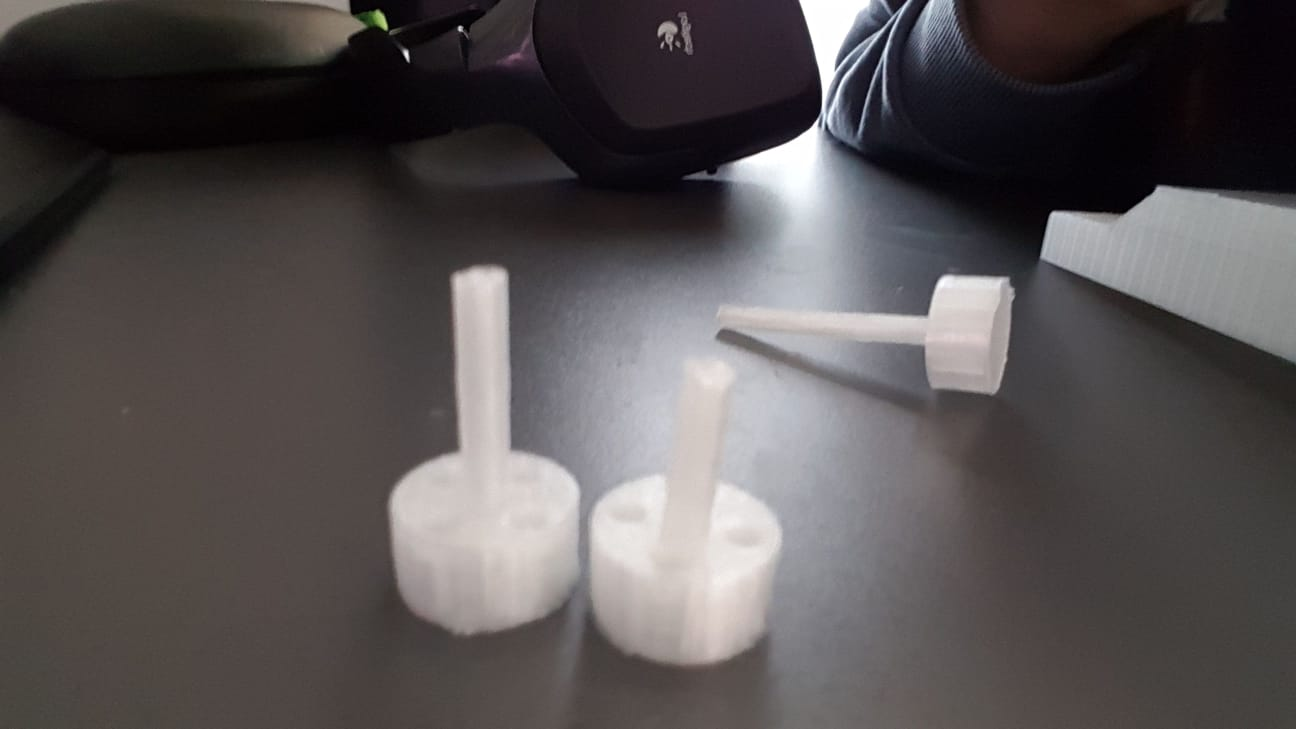
\includegraphics[
        width=0.5\linewidth,
    ]{imgs/no_enough_filling.jpg}
    \caption{Achsbruch durch Mangel an Füllmaterial}
    \label{fig-not-enough-filling}
\end{center}
\end{figure}
\noindent
Darüber hinaus konnte auch das Problem des Stützmaterials in eigentlich 
dringend benötigten Hohlräumen zur Befestigung noch nicht behoben werden.
Auch die in \ref{sec-ita2-visualization} beschriebene Lösung zur 
Darstellung der Emissionen ist in dieser Form noch nicht zufriedenstellend. Die Tests der Fahrzeugschaltung sind erfolgreich verlaufen und die Grundstruktur für den Programmablauf wurde implementiert.
\end{document}